\documentclass[12pt]{article}

\usepackage{upgreek}

\usepackage{amsmath}

\usepackage{dsfont}

\usepackage[utf8]{inputenc}

\usepackage{mathtools}

\usepackage{upquote}

\usepackage[english]{babel}

\usepackage{graphicx}

\usepackage{tikz}

\usepackage{hyperref}

\newcommand{\ts}{\textsuperscript}

\usepackage{tcolorbox}

\usepackage{amsthm,amssymb}

\setlength{\parindent}{0cm}

\renewcommand\qedsymbol{$\blacksquare$}

\usepackage{fancyhdr}

\usepackage{listings}
\usepackage{color}
 
\definecolor{codegreen}{rgb}{0,0.6,0}
\definecolor{codegray}{rgb}{0.5,0.5,0.5}
\definecolor{codepurple}{rgb}{0.58,0,0.82}
\definecolor{backcolour}{rgb}{0.95,0.95,0.92}
 
\lstdefinestyle{mystyle}{
    backgroundcolor=\color{backcolour},   
    commentstyle=\color{codegreen},
    keywordstyle=\color{magenta},
    numberstyle=\tiny\color{codegray},
    stringstyle=\color{codepurple},
    basicstyle=\footnotesize,
    breakatwhitespace=false,         
    breaklines=true,                 
    captionpos=b,                    
    keepspaces=true,                 
    numbers=left,                    
    numbersep=5pt,                  
    showspaces=false,                
    showstringspaces=false,
    showtabs=false,                  
    tabsize=1
}
 
\pagestyle{fancy}
\fancyhf{}
\fancyhead[LE,RO]{Machine Learning (Coursera) -- Summer 2017}
\fancyhead[RE,LO]{Joshua Concon}
\fancyfoot[CE,CO]{\leftmark}
\fancyfoot[LE,RO]{\thepage}


\begin{document}

\title{Machine Learning Lecture Notes}
\date{Stanford University (Coursera) -- Summer 2017}
\author{Joshua Concon}
\maketitle

Took this course on Coursera, taught by Andrew Ng. Note that I skip the linear algebra review as I already took a course relating to that topic. If you find any problems in these notes, feel free to contact me at conconjoshua@gmail.com.

\tableofcontents

\pagebreak

\section{Week 1}

\subsection{What is Machine Learning?}

Well besides being a buzzword this year, it's a "field of study that gives computers the ability to learn with being explicitly programmed" (quote by Arthur Samuel). A more rigorous definition given by Tom Mitchell would be "(a) Well-posed Learning Problem: A computer program is said to learn from experience $E$ with respect to some task $T$ and some performance measure $P$, if its performance on $T$, as measured by $P$, improves with experience $E$."\\
\\
In this course, we're gonna be learning about mainly supervised and unsupervised learning, but there are other types of Machine Learning algorithms such as Reinforcement Learning and Recommender Systems.

\subsection{Supervised Learning}

Supervised Learning is when an algorithm is already given the correct answers to a problem, and must generate more correct answers from the given info. Such an example can include classification algorithms that indicate the class of something by a different output (Like, 1 if a flower is a rose, 0 if a flower is a daisy). The algorithm would have to draw boundaries in the data for it to classify if a flower is a rose or a daisy from existing data of roses and daisies and would have to find patterns, and the number of features in the training examples being compared increases its accuracy.

\subsection{Unsupervised Learning}

Similar to Supervised Learning, but the right answers are not supplied and still the algorithm must create a structure. An example of this can be clustering algorithms where news articles are grouped based on the story that they cover, such as Google News.

\subsection{Model Representation (for Supervised Linear Regression)}

So here we are introduced to the mathematical models that will represent these algorithms, starting with supervised learning, where all the correct answers are given. Specifically for Linear Regression, we use this hypothesis function $$h(x) = \theta_0 + \theta_1 x = \hat{y}$$ where $x$ represents the input variables or features, $y$ represents the output variable or target variable and $\theta_0, \theta_1$ are just 2 constants. Further notation also includes $m$ as the number of training examples we have, $(x,y)$ as 1 training example and $(x^{(i)},y^{(i)})$ as the $i$\ts{th} training example.\\
\\
This hypothesis function is generated by our algorithm after our training sets have been fed into it. The generated $h$ function would then try to map the training example's $x$'s to their $y$'s.

\subsubsection{Cost Function}

Looking at the function $h$ graphed out, it will appear as different lines depending on the values of $\theta_0 \theta_1$, so generally we would want a line that is as close to the data as possible (that "fits" the data).\\
\\
To do exactly that, we would have to minimize the difference between the estimated $h(x)$ value and the actual $y$ value for each of the training sets, or to minimize
$$\frac{1}{2m} (h(x^{(i)}) - y^{(i)})^2\:\:\: \forall i, 1 \leq i \leq m$$

This is the square error function with the mean halved to make the computation of gradient descent easier (since we take the derivative of the function for gradient descent, and the derivative of the square function will cancel out with the $\frac{1}{2}$). So we are left with this cost function

$$J(\theta_0, \theta_1) = \sum^m_{i=1} \frac{1}{2m} (h(x^{(i)}) - y^{(i)})^2$$

\subsubsection{Intuition of the Cost Function}

Comparing the functions $h(x)$ and $J(\theta_0, \theta_1)$, $h$ is a function of $x$ for a fixed $\theta_0, \theta_1$, while $J$ is a function of $\theta_0, \theta_1$, and each value of $\theta_0, \theta_1$ changes $h(x)$ which changes how the $h(x)$ approximates data.\\
\\
And if you consider the contour plot or 3-D graph of $J$ with $\theta_0$ as the $y$ - axis and $\theta_1$ as the $x$ - axis, the graph as a minimum point at the most ideal line (since $J$ calculates error), and the ideal line would be a line with the smallest square error (i.e. a line that perfectly passes through all the points and $J(\theta_0, \theta_1) = 0$). The contour plot will tell you how far away the most ideal line is from the current line with a selection of $\theta_0$ and $\theta_1$.

\begin{figure}
  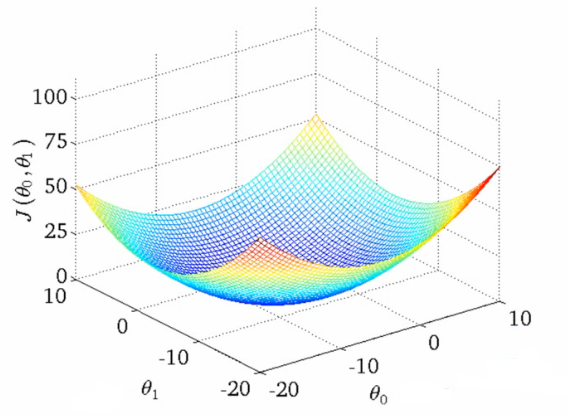
\includegraphics[width=\linewidth]{cost.png}
  \caption{Cost Function plotted on a 3-D graph (source: Stanford)}
\end{figure}

\subsubsection{Gradient Descent}

Gradient descent is actually more of a general algorithm used outside of Machine Learning, but we'll only learn of its ML applications.\\
\\
We will be using Gradient Descent to estimate the ideal parameters $\theta_1, \theta_0$ for $J$ to get the minimum value. More specifically, we'll be starting off with generic values for $\theta_1, \theta_0$ and it would continue to change them in a way that $J$ would always decrease until $J$ reached the global minima. If you refer to the graph posted before, you'll notice that $J$ also has one minima, so we can be sure that gradient descent approaches an ideal line if we keep moving in the direction of greatest decrease. To find the direction of greatest decrease, we take the derivative at that point, and we move by a step size of $\alpha$ each time, which is called the learning rate.\\
\\
So the algorithm for gradient descent would look something like the code posted above.

\begin{figure}
  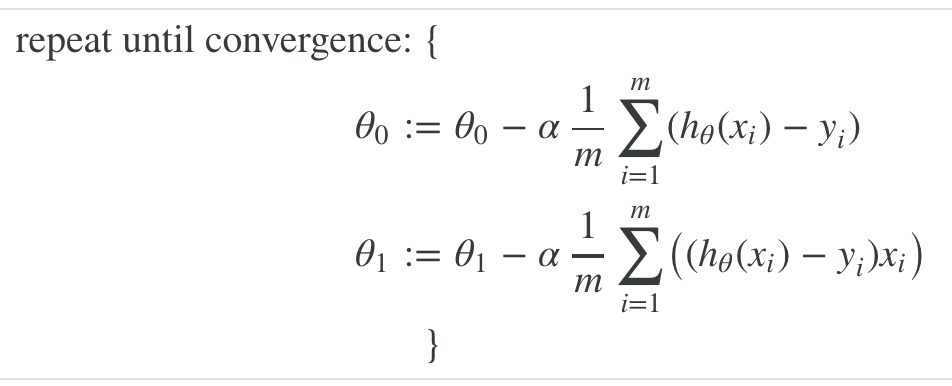
\includegraphics[width=\linewidth]{GD.png}
  \caption{Sudo Code for Gradient Descent (source: Stanford)}
\end{figure}

\underline{Note:} that all variables must be updated simultaneously at the very end of each loop and not in-between the loop.\\
\\
We can also tell if the algorithm has converged if the derivative is 0 (i.e. the next step does not change the points $\theta_1, \theta_0$).\\
\\
However, the learning rate $(\alpha)$ cannot be too big or too small. Too small and it will converge in too many steps, and too big and the algorithm can overshoot the minima and fail to diverge.


\end{document}